%----------------------------------------------------------------------------
\chapter{Az elvégzett munka}
%----------------------------------------------------------------------------

(40 oldal)

%----------------------------------------------------------------------------
\section{Rendszerterv}
%----------------------------------------------------------------------------
\begin{figure}[!ht]
\centering
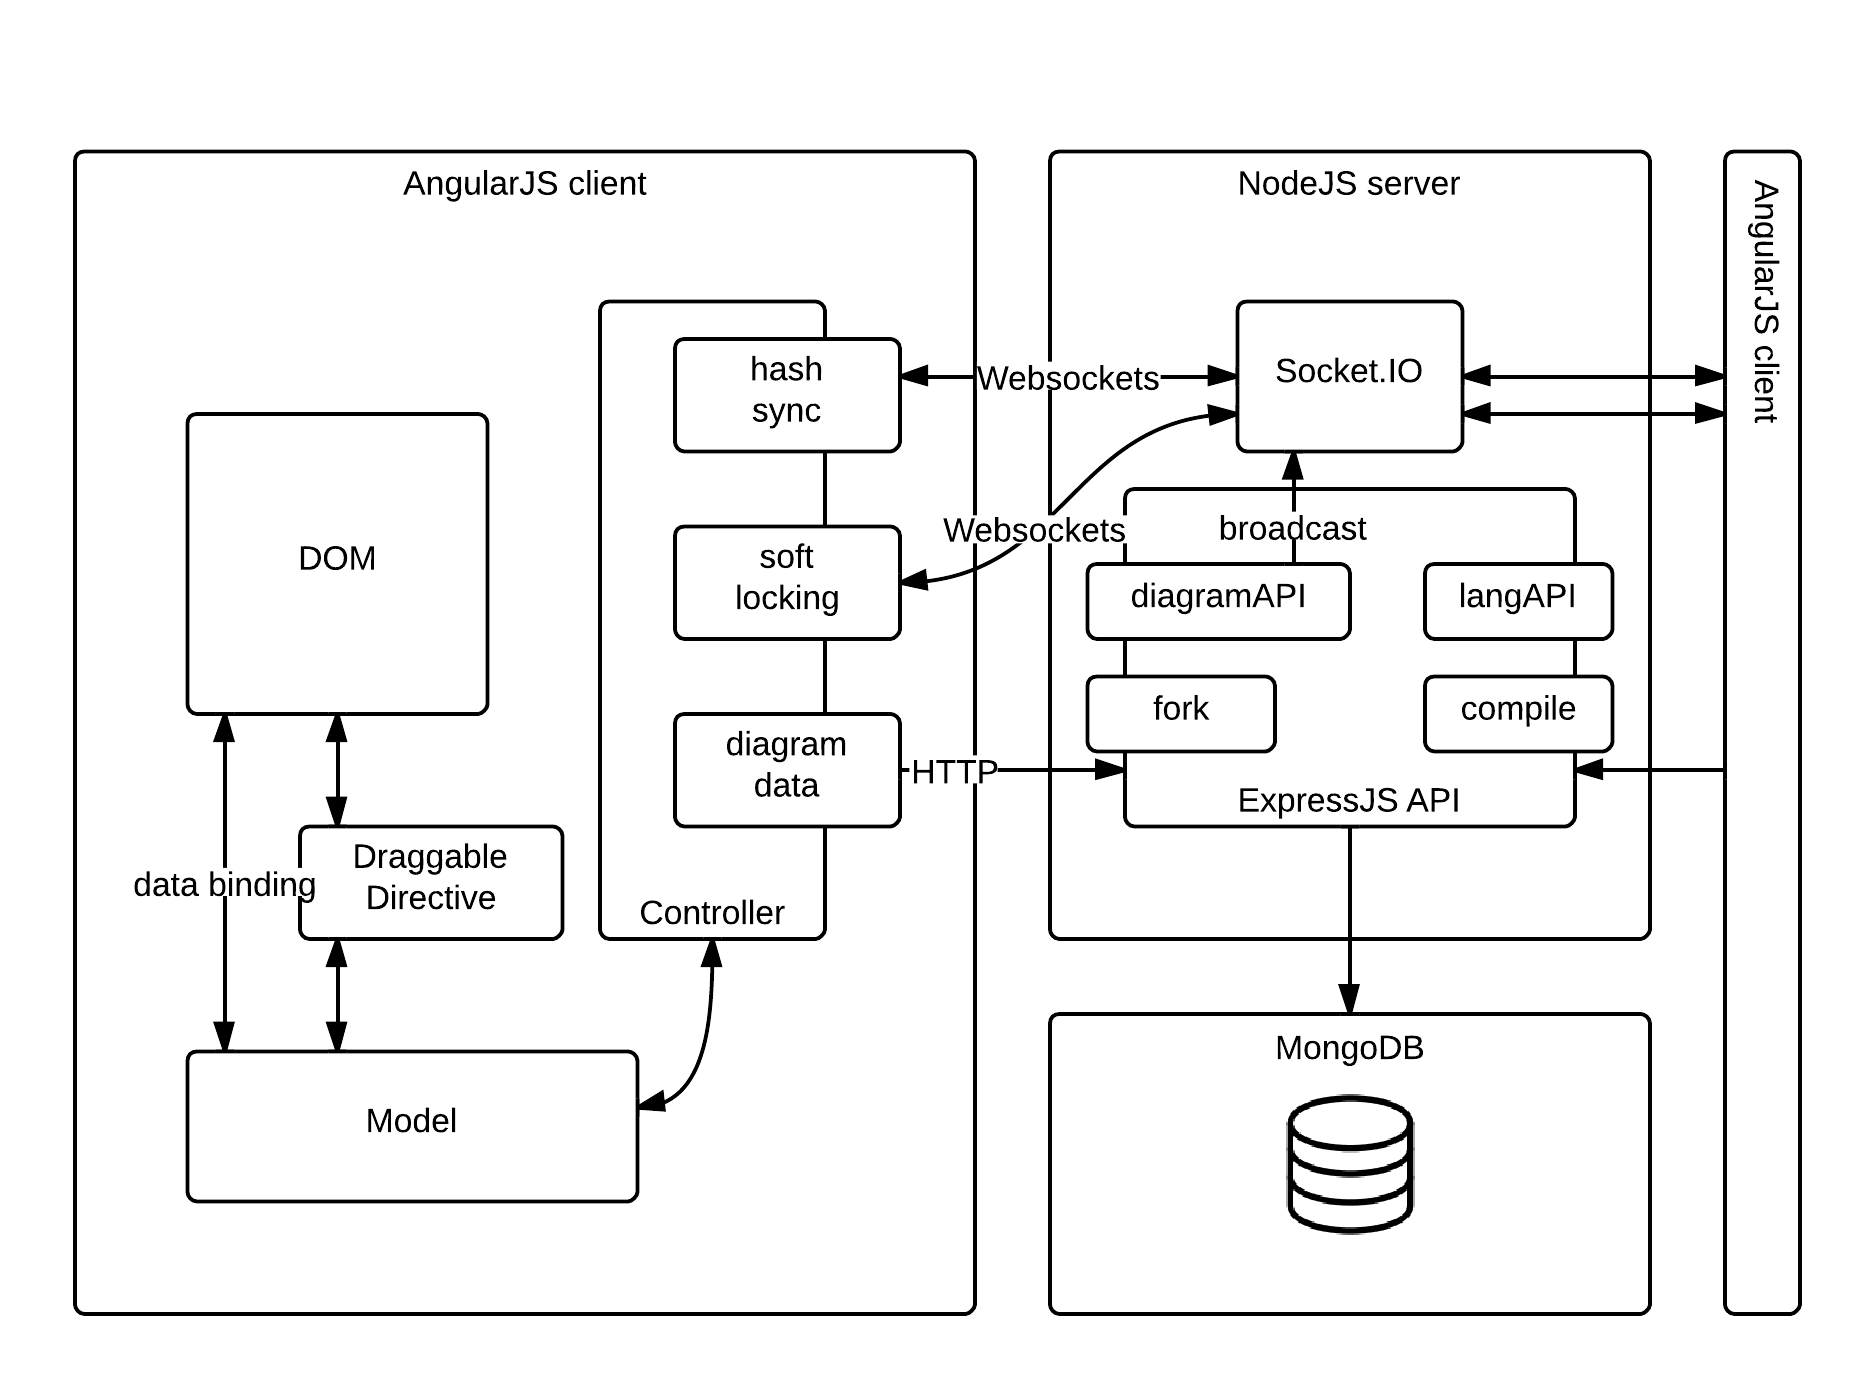
\includegraphics[width=100mm,keepaspectratio]{figures/Rendszerterv.png}\\
\end{figure}

\subsection{Kollaboráció}

Mivel kollaboratív alkalmazásról van szó elsőbbségi szempont az ellentmondó, nagyjából egyidejű változtatások konfliktusait feloldani. Felmerült ötletként a Google Docs-ban alkalmazott Operational Transformation megoldás amiben folyó szöveg egyidejű módosítása van megoldva ``előbb-útóbbi'' konzisztencia elérésével. Az Operational Transformation algoritmust nehéz implementálni CITATIONNEEDED, viszont vannak nyílt forráskódú megoldások rá\footnote{http://www.sharejs.com}. Nem ezen a vonalon indultam el, mert nehézkesnek gondoltam annak a rétegnek a fejlesztését ami a DOM-ban levő gráfot szöveggé- és vissza transzformálja akkor is , ha meg van oldva a különböző kliensek által látott szövegreprezentáció kollaboratív változtatása. 

Erre az alternatíva ami végül kiválasztásra került egy meglehetősen pehelysúlyú megoldás: a gráf módosítását jól meghatározott eseményekként defineálom és ezek az események a többi felhasználóhoz Websockets broadcast üzeneteken keresztül jutnának el. Egy példa esemény egy entitás módosítása: az A kliens böngészőjében elhúzunk egy dobozt, a kliensoldali kód a szervernek egy kérésben szól a módosításról, a szerver perzisztálja az adatot és Websockets broadcast üzeneten keresztül értesíti a többi résztvevőt. Ilyenkor az esemény üzenet az új értékét is tartalmazza az entitásnak ami módosult. 

Ebben a megoldásban igazából semmi konfliktus feloldás nincsen és a továbbiakban be fogom mutatni, hogy ez nem is feltétlenül szükséges. Először is nézzük meg, hogy milyen jellegű konfliktusokról lehet szó; a közösen manipulált elemeket lehet egyidejűleg létrehozni, törölni és módosítani, feltételezve két szereplőt a következő esetek relevánsak:

\begin{enumerate}
\item { törlés - törlés} Ha majdnem egyszerre ketten törlik ugyanazt az entitást, akkor csak kezelni kell kliens és szerver oldalon, hogy a később érkező törlés művelet már fölösleges. 
\item { módosítás - módosítás} Itt két eset lehetséges:
\begin{enumerate}
\item Különböző attribútumok változnak. Ekkor, ha csak a változásokat küldjük el , akkor ????összefésülhetők az attribútumok, ha nem , akkor igazából a következő esetről beszélünk,
\item Ugyanazok az attribútumok változnak. Ekkor sajnos arról beszélünk, hogy egyidejűleg az első felhasználó jobbra 
húzta , a másik felhasználó balra húzta az objektumot és a később történt esemény fog végül érvényesülni. 

Az első kérdés ami felmerül itt az, hogy ez egyáltalán próbléma? Próbléma, mert a mozgatás elvesztése apró művelet könnyen megismételhető, de ha egy hosszú szöveg beírásáról van szó egy attribútum mezőbe, akkor nem kívánatos elveszíteni azt. Egyszerű modellek szerkesztésénél mint egy állapot diagram nem tipikus a hosszú szövegek beírása. 

Jó esetben körülbelül 100 ms alatt mindenkihez eljutnak az események, ez azt jelentené, hogy nem lehet annyira gyakori ez a próbléma, hogy egy verziókezelő rendszerhez hasonló megoldással lassítsuk a felhasználók munkafolyamatát.

\pdfcomment[icon=Note]{insert: Zárolás}

Egy egyszerű felhasználói élmény javítás egy jelzés lesz, ami úgy néz ki, hogy minden felhasználó látja, hogy ki éppen milyen objektumot jelölt ki színekkel jelölve. Ha valaki más ki szeretné törölni az objektumot aminek az életrajzát éppen írjuk, akkor a rendszer legalább szól, hogy azt valaki kijelölte. Ez a megoldás egyik fő előnye, hogy nem bonyolítja egyáltalán a munkafolyamatot példáúl a zároláshoz képest.

\end{enumerate}
\item { módosítás - törlés } Ez a szituáció ugyanaz mint az előző. A fent említett megjelölés egy megoldás, de egy visszavonás művelet megnövekedett komplexitás árán megoldaná teljesen a próblémát.
\end{enumerate}

\pdfcomment[icon=Note]{insert: A többi miért irreleváns?}

Ha a két művelet két különböző csúcsot érint, akkor nincs próbléma, mert triviálisan mindkét művelet érvényesül, ha a egy csúcsot és egy hozzá tartozó élet érint, akkor sincs gond, mert a csúcs törlése maga után vonja az él törlését is. 

Az 5FEJEZET-ben teljesítményelemzés keretein belül további indoklást részletezek. 

Az előnye a megoldásnak az egyszerűség és a remélhetőleg jobb felhasználói élmény ami abból eredhet, hogy visszaigazolás nélkül módosul a felhasználó felületén a diagram a saját beavatkozása után. Egy olyan alkalmazásnál ami egy nem-kollaboratív offline alkalmazással versenyzik létfontosságú a kis reakcióidő a felületen. Az egyszerűség maga után vonja a könnyebb karbantarthatóságot és kisebb hibalehetőséget.   


Egy hátránya az, hogy az események száma nő a komplexitás növekedésével. 



\subsubsection{Eltérések detektálása}

Egy funkció ami jelzi, hogy két felhasználó eltérő diagramot lát holott ugyanazt kellene, hogy lássák -- nevezzük eltérés detektálásnak -- két szempontból is hasznos lesz: egyrészt a teljesítményelemzés során fel lehet használni arra, hogy a kollaborációs megoldás hatékonyságát vizsgáljam különböző paraméterek mellett , másrészt felhasználói élmény szempontjából szükséges, hiszen, ha eltérést vesz észre az algoritmus, akkor a diagram újratöltésével orvosolható a próbléma. 
A kérdés az, hogy mi az amit összehasonlítunk ilyenkor? A teljesítményt és a sávszélességet szem előtt tartva egy egyszerű megoldás egy hash értéket számolni a diagramból majd ezt összevetni a többi kliens által kiszámolt értékkel.

Ux

Szerver is részt vesz?

Teljesítmény

Nyugtázás?

Másik kérdés, hogy, hogyan oldható meg az, hogy ugyanabban az időben normális körülmények között előfordulhat, hogy 



%----------------------------------------------------------------------------
\section{Adatbázis}
%----------------------------------------------------------------------------

A kliens oldalról nézve egy felhasználói diagram fő elemei az entitások és a köztük lévő kapcsolatok (vagy csúcsok és élek a gráfban). 


\begin{lstlisting}
{
    "_id" : ObjectId("52486e8e9b7f14a725000001"),
    "position" : {
        "top" : 312.9618225097656,
        "left" : 607.920166015625
    },
    "title" : "Alszik",
    "document" : "5242aa48ddda9b0000000001"
}
\end{lstlisting}

Az entities kollekcióban tárolva vannak a diagram entitásai. Lehetne egy kollekcióban tárolni mindent ami egy diagramhoz tartozik, de azért van szükség külön kollekcióban tárolni az entitásokat, mert az egyedi azonosítójukra szükség van a kliens oldalon is. ERROLBOVEBBENAKLIENSOLDALIALKALMAZASBAN
A position attribútum konkrétan a kliensoldali CSS pozícionálásra van használva, a document attribútum egy idegen kulcs lenne, ha relációs adatbázisról beszélnénk, de valóban annak a dokumentumnak az azonosítóját tárolja aminek része.

\begin{lstlisting}
{
    "_id": "524b08b1b7f4db8e68000001",
    "connections": [
    {
        "from": "524b08b4b7f4db8e68000002",
        "to": "524b08bdb7f4db8e68000003",
        "label": "valami"
    },
    ...],
    "entities": [],
},
\end{lstlisting}


%----------------------------------------------------------------------------
\section{A szerver oldali alkalmazás}
%----------------------------------------------------------------------------






%----------------------------------------------------------------------------
\subsection{Kétirányú kommunikáció}
%----------------------------------------------------------------------------

Ha azt nézzük, hogy egyidejűleg x darab diagramot szerkeszt diagramonként y darab különböző felhasználó, akkor felmerül az a próbléma, hogy hogyan követjük nyomon, hogy milyen eseményeket milyen socket-ekre kell továbbítani, más szóval hogyan történjen a broadcast. Szerencsére a Socket.IO könyvtár ezt megoldja úgynevezett szoba funkcionalitással, egy szobához hozzáadott socketek tudnak broadcast üzenetet küldeni a többi szobabeli socketnek, ráadásul a socketek eltávolítása is átlátszóan történik és nem kell memóriakezelési próblémákkal küzdeni.Így a socket kezelő szerver oldali logika meglehetősen vékony lesz, de ez is a célja a Socket.IO könyvtárnak. 

Mivel minden szerkesztendő diagramhoz tartozik egy szoba, kézenfekvő a diagram azonosítóját beállítani a szoba neveként. A modularitást szem előtt tartva, a socket kezeléssel kapcsolatos funkcionalitást egy SocketAdapter nevű objektumba csomagoltam. A SocketAdapter példány példányosítja a Socket.IO szervert és gondoskodik az új kapcsolatok beállításáról, rajta keresztül lehet hívni Socket.IO függvényeket.

Egy új socket-re eseménykezelőket hoz létre a SocketAdapter és a legfontosabb talán a \lstinline{room:change} esemény, ami egy diagram megnyitásakor, vagy másik diagram-ra való áttéréskor hívódik meg a kliens által. Ekkor a régi szobából átkerül az új szobába a socket. 

\begin{figure}[!ht]
\centering
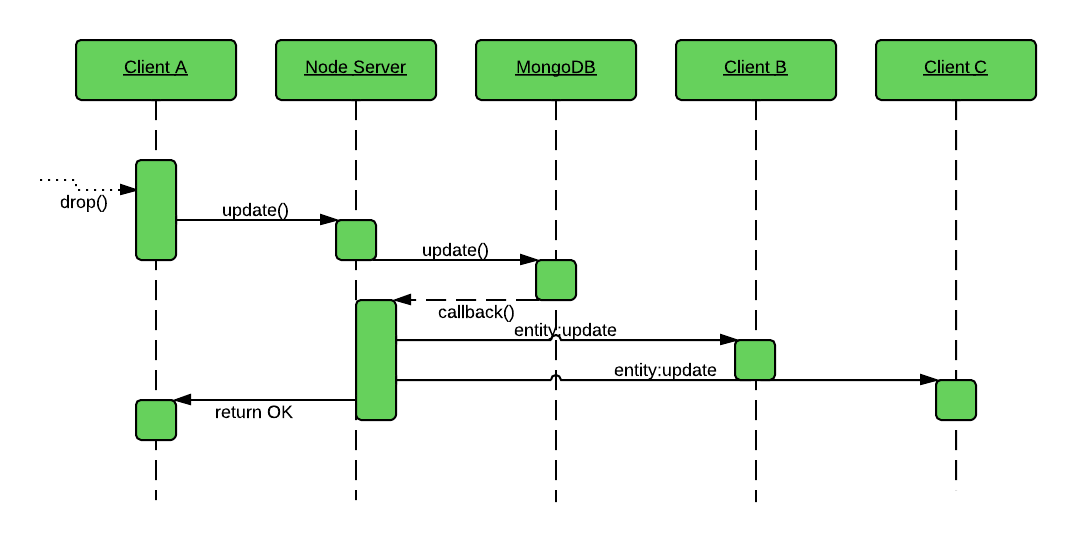
\includegraphics[width=15cm,keepaspectratio]{figures/collaboration-seq.png}
\caption{Entitás módosítás feldolgozása}
\label{fig:angularhtml}
\end{figure}




%----------------------------------------------------------------------------
\section{A kliens oldali alkalmazás}
%----------------------------------------------------------------------------
Derp.




%----------------------------------------------------------------------------
\subsection{Szolgáltatások}
%----------------------------------------------------------------------------


\begin{lstlisting}
  app.factory('DocumentService', ['$resource', function($resource){
  return $resource('/api/docs/:id', {id:'@_id'}, 
    { update: {method:'PUT' } , 
      query: {method:'GET', isArray: true}});
    }]);
\end{lstlisting}


%----------------------------------------------------------------------------
\subsection{Unit teszt esetek}
%----------------------------------------------------------------------------



%----------------------------------------------------------------------------
\section{Pehelysúlyú zárolás}
%----------------------------------------------------------------------------

Ahelyett, hogy megakadályozzam, hogy a többi résztvevő felhasználó, ne változtathassák bizonyos részeit a diagramnak, csak egy jelzési mechanizmust implementáltam, amivel láthatóvá válik, ha valaki kijelölt egy entitást. Ehhez először szükség van a szoba résztvevők nyilvántartására, hiszen a kollaborációhoz nem volt kötelező tudni, hogy ki nézi még a diagramot.

Szerencsére szerveroldalon a Socket.IO könnyen elérhetővé teszi ezt az információt: \lstinline{io.sockets.clients(szoba);} egy socket objektumokból álló tömböt ad vissza. A \lstinline{connection} és a \lstinline{disconnect} események hatására értesül a szerveroldal arról, hogy valaki kapcsolódott, vagy elhagyta a szobát.

\begin{figure}[!ht]
\centering
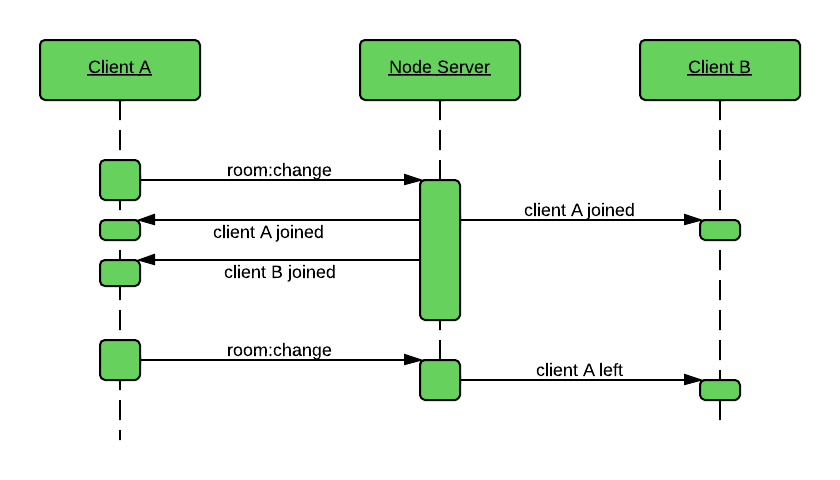
\includegraphics[width=15cm,keepaspectratio]{figures/join-seq.png}
\caption{Felhasználó belép a szobába}
\label{fig:joinseq}
\end{figure}

Az ábrán látszik, hogy szoba váltáskor a szerveroldal minden résztvevőjét a szobának (az új résztvevőt beleértve) értesít arról, hogy belépett, és az új résztvevőnek a létező socketek listáját is elküldi. Kilépéskor vagy diagram váltáskor is értesíti a klienseket. Így a kliensek nyilvántartást tudnak tartani a kapcsolódott többi kliensről. A \lstinline{client joined} és a \lstinline{client left} üzenetek esetében -- mivel az alkalmazás nem használ felhasználói fiókokat -- egy socket példány azonosítót is küld a kliensnek.

A socket azonosítókhoz színeket lehet nagyon egyszerűen rendelni úgy, hogy md5 hash-t számoltatok az azonosítóból és így egy hexadecimális értéket kapok. Ennek elég 6 betűjét venni és már megvan egy -- nagy valószínűséggel -- egyedi szín, legalábbis egy megnyitott diagramon belül.

Ez a jelölés a ~\ref{fig:entitydir} ábrán is látszik. 

A jelöléseket egy kulcs-érték objektum tartalmazza, a kulcs az entitás azonosító, az érték az felhasználó színazonosítója. Ez a reláció irány azért hasznos, mert az entitás direktíva közvetlenül tud erre a színre hivatkozni:

\begin{lstlisting}
 <div class='entity_mark' style='background-color:#{{marks[entity._id]}};'>
 </div>
\end{lstlisting} 

tehát, ha van az objektumban egy konkrét entitás azonosító mint kulcs, akkor megjelenik egy olyan színű doboz, ha nem, akkor nem látszik semmi. 

Viszont, amikor egy másik kliens jelöléséről értesülünk, akkor egy entitás azonosítót és egy kliens azonosítót kapunk, ekkor nagyon kézenfekvő lenne a fordított irányú kulcs-érték objektum, vagyis kliens azonosítókhoz rendelt entitás azonosító. Ha ez meglenne, akkor egy műveletben kicserélnénk a régi jelölését az újra. Szerencsére az underscoreJS eszközkészletében találunk dictionary megfordítót:

\begin{lstlisting}
    socket.on('mark', function (data) {
        var inverted = _.invert($scope.marks)
        // user->id
        $scope.marks[inverted[data.user]] = null;
        $scope.marks[data.id] = data.user;
    });
\end{lstlisting}

Itt látszik, hogy ez a broadcast is szokásosan Socket.IO segítségével történik.


\section{Vizuális programozási nyelvek és kódgenerálás}

\begin{figure}[!ht]
\centering
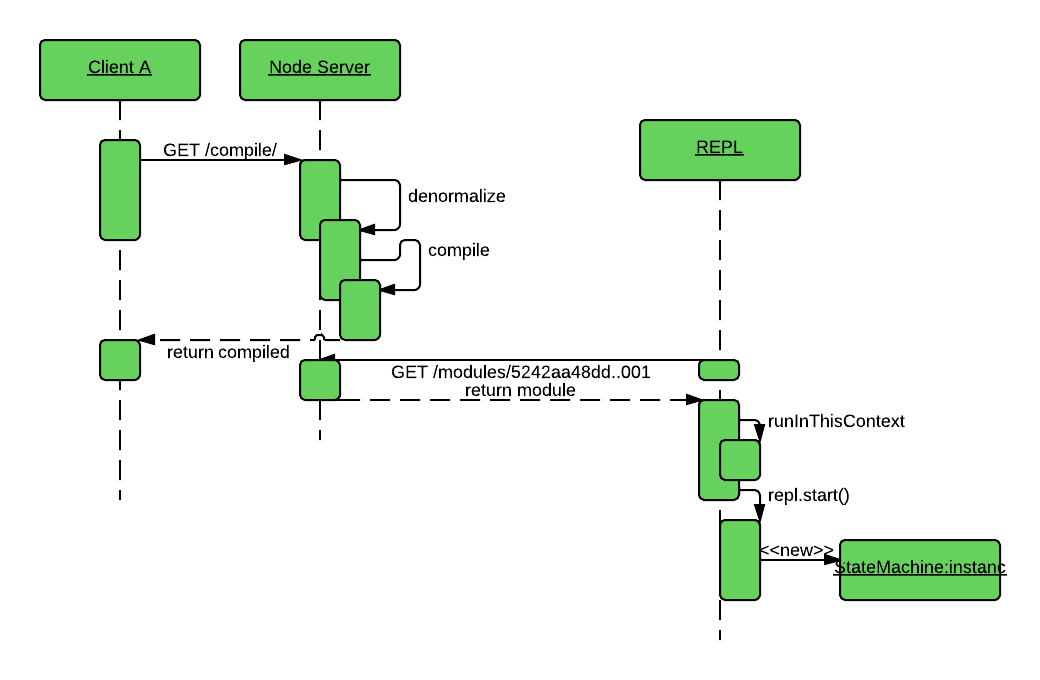
\includegraphics[width=15cm,keepaspectratio]{figures/compile-seq.png}
\caption{Kódgenerálás}
\label{fig:compileseq}
\end{figure}

A kollaboratív gráfszerkesztésen túl az alkalmazás egyszerű vizuális programozási nyelvek létrehozására alkalmas.
A vizuális programozás menete a következő egy minta nyelv példányán amiben állapotgépeket lehet programozni:
\begin{enumerate}
\item A kliensoldalon a felhasználó elkészíti a gráftranszformációs template kódot,
\item A felhasználó elkészíti egy vizuális implementációját a nyelvnek, vagyis egy konkrét állapot gépet vizuálisan,
\item A fordítás gomb megnyomása után a szerveralkalmazás denormalizálja a gráfot, azaz létrehoz egy olyan struktúrát, ami a diagramot reprezentálja redundánsan. Ez a struktúra a bemenő adata a gráftranszformáló template-nek,
\item A szerveralkalmazás a template alapján egy konkrét állapotátmenetekkel rendelkező állapotgép Javascript kódját hozza létre,
\item Ezt a kódot elmenti az adatbázisba és választ küld a kliensalkalmazásnak, ekkor kétféleképpen lehet felhasználni a kódot:
\begin{enumerate}
    \item A felhasználó böngészőjének Javascript parancssorában (példáúl Chrome Developer Console) értelmezi a kódot \lstinline{eval} segítségével és példányosítja az állapotgépet. 
    \item Node.JS parancssorból a mintrepl segédalkalmazással betölti a kódot, majd példányosítja az állapotgépet.
\end{enumerate}
\end{enumerate}


\subsubsection{Denormalizálás}

Az eredeti ``séma'' csúcsok listáját és élek listáját jelenti, viszont ez az adatformátum nem hasznos relációk kezelésére. Ezért reláció helyett redundancia bevezetésével oldom meg: egy diagram ilyen reprezentációjában egy él többször is jelenik meg. Ez leegyszerűsítve így néz ki:

\begin{lstlisting}
    {   edges: [
            {from: a, to: b},
            {from: a, to: c}],
        points: [
            {name: a, outgoing: [{from: a, to: b},{from: a, to: c}], incoming: []},
            {name: b, outgoing: [], incoming: [{from: a, to: b}]},
            {name: c, outgoing: [], incoming: [{from: a, to: c}]},
        ]
    }
\end{lstlisting}

Így ezen a struktúrán kevesebb kóddal írható egy olyan transzformáció ami valamilyen logikát valósít meg abból kiindulva, hogy milyen állapotból milyen élek mennek ki és be. Ez struktúra ami ilyenkor létrejön csak átmenetileg van felhasználva amíg kódot generál a szerveroldal, utána nem lesz használva semmire, így nem kella redundancia által okozott szokásos próblémákkal küzdeni. Ebben a formában tárolni mindig a gráfot nem hatékony, mert minden diagram manipulációs művelet több mint egy adatbázis lekérdezést jelentene és ha el szeretném kerülni a redundancia anomáliákat 
akkor megnövekedne fölöslegesen a komplexitás (tranzakciókra lenne szükség, vagy zárolásra és ezeket nem biztosítja a MongoDB). Ez a denormalizálás viszont csak két for ciklusból áll és ritkán fut le. 

\subsubsection{Gráftranszformáció template}

A gráftranszformáció template egy Underscore template. Underscore.JS egy Javascript könyvtár ami funkcionális programozás eszközökkel bővíti e nyelvet, anélkül, hogy kiterjesztené a beépített típusokat. \cite{underscorejs.org}
Ezen belül a template rendszer lehetővé teszi egy template fájlt lefordítását adott kontextus alapján. A template-ben \lstinline{<\%= \%>} segítségével változó behelyettesítés történik, \lstinline{<\% \%>} segítségével Javascript kódot lehet értelmeztetni. 

\begin{lstlisting}
var compiled = _.template("hello: <%= name %>");
compiled({name: 'moe'});
=> "hello: moe"
\end{lstlisting}

Az alkalmazásban így néz ki felhasználói szemszögből:

\begin{figure}[!ht]
\centering
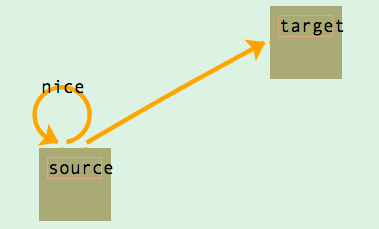
\includegraphics[width=5cm,keepaspectratio]{figures/simple-graph.png}
\caption{Egy példa diagram}
\label{fig:compileseq}
\end{figure}

\begin{lstlisting}[caption=A template]
Elements: 
<% 
    doc.entities.forEach(function(el){
%>
    <%= el.title %>
<%
    })
%>
\end{lstlisting}

És a kimenet: 
\begin{lstlisting}[language=HTML]
Elements: 

source
target
\end{lstlisting}

Természetesen nem csak Javascript kódot lehet generáltatni az alkalmazásban, hiszen a template behelyettesítés eredménye egyszerű szöveg. 






%---------------------------------------------------
\subsubsection{A generált kód felhasználása}
%---------------------------------------------------

A generált kód elmentődik az adatbázisba a diagram egyik attribútumába, és ehhez az adathoz egy API végponton keresztül lehet hozzáférni és felhasználni meg akár a triviális HTML script elem segítségével:

\begin{lstlisting}[language=HTML]
 <script type="text/javascript" src="http://localhost:3000/api/compile/modules/5242aa48ddda9b0000000001/"></script>
\end{lstlisting}

Parancssorból is fel lehet használni \lstinline{node mintrepl <id>} segítségével, a mintrepl egy javascript szkript, ami a fent említett API-n keresztül letölti és értelmezi a fájlt, majd futtatja a letöltött kódot és egy REPL\footnote{Read-Eval-Print-Loop} interaktív node shell-t futtat. 

\begin{lstlisting}
 $ node mintrepl 5242aa48ddda9b0000000001
 mint 5242aa48ddda9b0000000001> tanulo = new sm()
 mint 5242aa48ddda9b0000000001> tanulo.consumeEvent("kávé")
 mint 5242aa48ddda9b0000000001> tanulo.currentState
 ébren
 \end{lstlisting}

 Hasonló módon egy másik node szerver szerveroldali kódjába is be lehet illeszteni. 
 










%----------------------------------------------------------------------------
\section{A Websockets protokoll vizsgálata}
%----------------------------------------------------------------------------

A Wireshark csomagvizsgáló eszközzel megvizsgáltam jobban a websockets kommunikációt.  




%----------------------------------------------------------------------------
\section{Promises és a ``callback hell''}
%----------------------------------------------------------------------------
Derp.


